\documentclass[10pt,conference,compsoc,letterpaper]{IEEEtran}
\usepackage[T1]{fontenc}
\usepackage{microtype}
\usepackage{amsmath,amssymb}
\usepackage{booktabs}
\usepackage{graphicx}
\usepackage{tikz}
\usetikzlibrary{arrows.meta,positioning,calc}
\usepackage{cite}
\usepackage[hidelinks]{hyperref}
\hypersetup{pdftitle={From a Sentence to an Annealer: Local-LLM Agents for Data-Grounded QUBO Optimization},pdfauthor={Chia Chen Yang},pdfsubject={QCNC conference manuscript}}
\title{From a Sentence to an Annealer: Local-LLM Agents for Data-Grounded QUBO Optimization}
\author{\IEEEauthorblockN{Chia Chen Yang}}
\begin{document}
\maketitle
\begin{abstract}
Turning a natural-language request into an annealing result requires more than a valid quadratic unconstrained
binary optimization (QUBO) formula. Public data must be acquired and interpreted, the model must preserve the
confirmed requirements, and the delivered decision must be checked independently of its QUBO energy.
We present a human-in-the-loop workflow in which locally served language-model agents clarify requirements,
generate a binary model, acquire and preprocess data, and submit QUBOs to interchangeable classical,
quantum-inspired and hybrid backends. Typed data interfaces, separate data and requirement checkers, and bounded
cross-stage repair provide executable feedback. We also replace reference-bitstring verification with a
problem-level protocol that checks every decoded ground state against a benchmark-anchored evaluator.
An audit found incorrect generated test cases in at least seven of twelve shape failures. Across three runs on
100 benchmarks, problem-level verification yielded 69, 72 and 70 successes; 27 benchmarks changed outcome.
A synthetic 12-category suite produced valid models in all 36 runs. Fixed-model comparisons returned feasible
solutions in all 54 simulated-annealing/GPU conditions and all 27 D-Wave Leap Hybrid conditions, with an explicit
ten-second Hybrid limit. Specified-source real-data pilots establish narrower integration capabilities;
autonomous public-data acquisition and the incremental effects of checkers, repair and retrieval remain to be
evaluated under a frozen repeated protocol. The contribution is a data-grounded workflow and evaluation methodology that distinguishes data and modelling
errors from solver limitations.
\end{abstract}

\begin{IEEEkeywords}
QUBO, local language models, agent workflows, problem-level verification, hybrid quantum-classical optimization
\end{IEEEkeywords}
\section{Introduction}
Quadratic unconstrained binary optimization (QUBO) provides a common input for quantum annealers,
quantum-inspired devices and hybrid services. Formulations exist for many combinatorial problems\cite{lucas2014ising}.
However, a person asking where to install charging stations or how to organize an inspection route does not
start with a QUBO matrix. Their request must be clarified, relevant data found and cleaned, a formulation
written, solver resources allocated, and the returned decision explained. Errors at any stage can yield a
feasible solution to a different problem.

Language models can assist this translation. NL4Opt studies natural-language optimization
representations\cite{ramamonjison2023nl4opt}; OptiMUS formulates and solves mixed-integer linear
programs\cite{ahmaditeshnizi2024optimus}. QuantumQUBO Agent decomposes QUBO generation into specialized roles
and evaluates generated formulations on a 100-problem benchmark\cite{mondal2026quantumqubo}.
LLM-QUBO combines language-based formulation with hybrid decomposition\cite{llmqubo2025}.
These lines of work motivate separating modelling from execution and checking. Our focus is the surrounding
workflow: whether the data represents the request, whether the model preserves its requirements, and whether
its output is a usable decision.

The distinction matters in public-data applications. Two tables can use different coordinate systems or spell
the same administrative unit differently. A join by village name can discard entities when names recur across
districts. Separately, a model may enforce a bound of 200 where the user requested five facilities.
Increasing penalties cannot restore missing entities or correct that bound. Consequently, solver feedback must
be interpreted alongside data and formulation evidence before deciding where to repair.

We study the following question: \emph{How can a locally served LLM, supported by specialized roles and executable
feedback, take a confirmed request through data preparation, modelling and annealing while making failures
observable and recoverable?} The operational goal is a feasible, interpretable decision within a bounded budget,
or a concrete explanation of the unresolved gap. A certified optimum is not required for every application.
People confirm the specification, approve data assumptions and review delivery.

Our contributions are threefold:
\begin{enumerate}
  \item A local-LLM workflow with typed data interfaces, tool-supported acquisition and preprocessing,
        versioned artifacts, interchangeable annealing backends and bounded cross-stage repair.
  \item A verification design that separates data correctness, requirement consistency and solver feasibility.
        For small benchmark instances, decoded ground states are evaluated against a checker anchored on the
        benchmark's stated optimum, avoiding dependence on a particular bit layout.
  \item An evidence-separated evaluation: repeated formulation benchmarks, a synthetic end-to-end suite,
        fixed-model backend experiments and specified-source real-data pilots. An implemented autonomous
        acceptance protocol defines the remaining checker, repair and modelling-retrieval comparisons.
\end{enumerate}
The solver-side components reuse established software and encoding methods rather than introduce a new penalty
search algorithm. More agent roles or retrieved patterns are not assumed to help; their incremental effects
require controlled measurements.

\section{Workflow and Validation Interfaces}
\label{sec:system}
\subsection{Problem and delivery contract}
A confirmed specification $s$ defines an original objective $f_s(x;d)$ and constraints $c_j(x;d)$ over prepared
data $d$ and binary decisions $x$. After converting the objective to minimization, the compiler builds
\begin{equation}
 E_{\lambda}(x,z;d)=f_s(x;d)+\sum_j\lambda_j P_j(x,z;d),
\end{equation}
where $z$ contains encoding auxiliaries and $P_j$ is the selected constraint penalty. Changing $\lambda$ changes
QUBO energy, so different configurations are ranked by original-constraint feasibility and objective, not raw
energy. Approximate encodings are identified explicitly.

Inputs are classified as public facts, user settings or private data. Public fields require source records;
settings are confirmed rather than searched for. Private inputs must be provided or explicitly marked as mock.
The output includes the specification, prepared data and provenance, model, solution, figure and assumptions.
Delivery states whether the solution came from annealing or a conventional baseline, and distinguishes usable,
limited-quality and unavailable outputs.

\begin{figure*}[t]
\centering
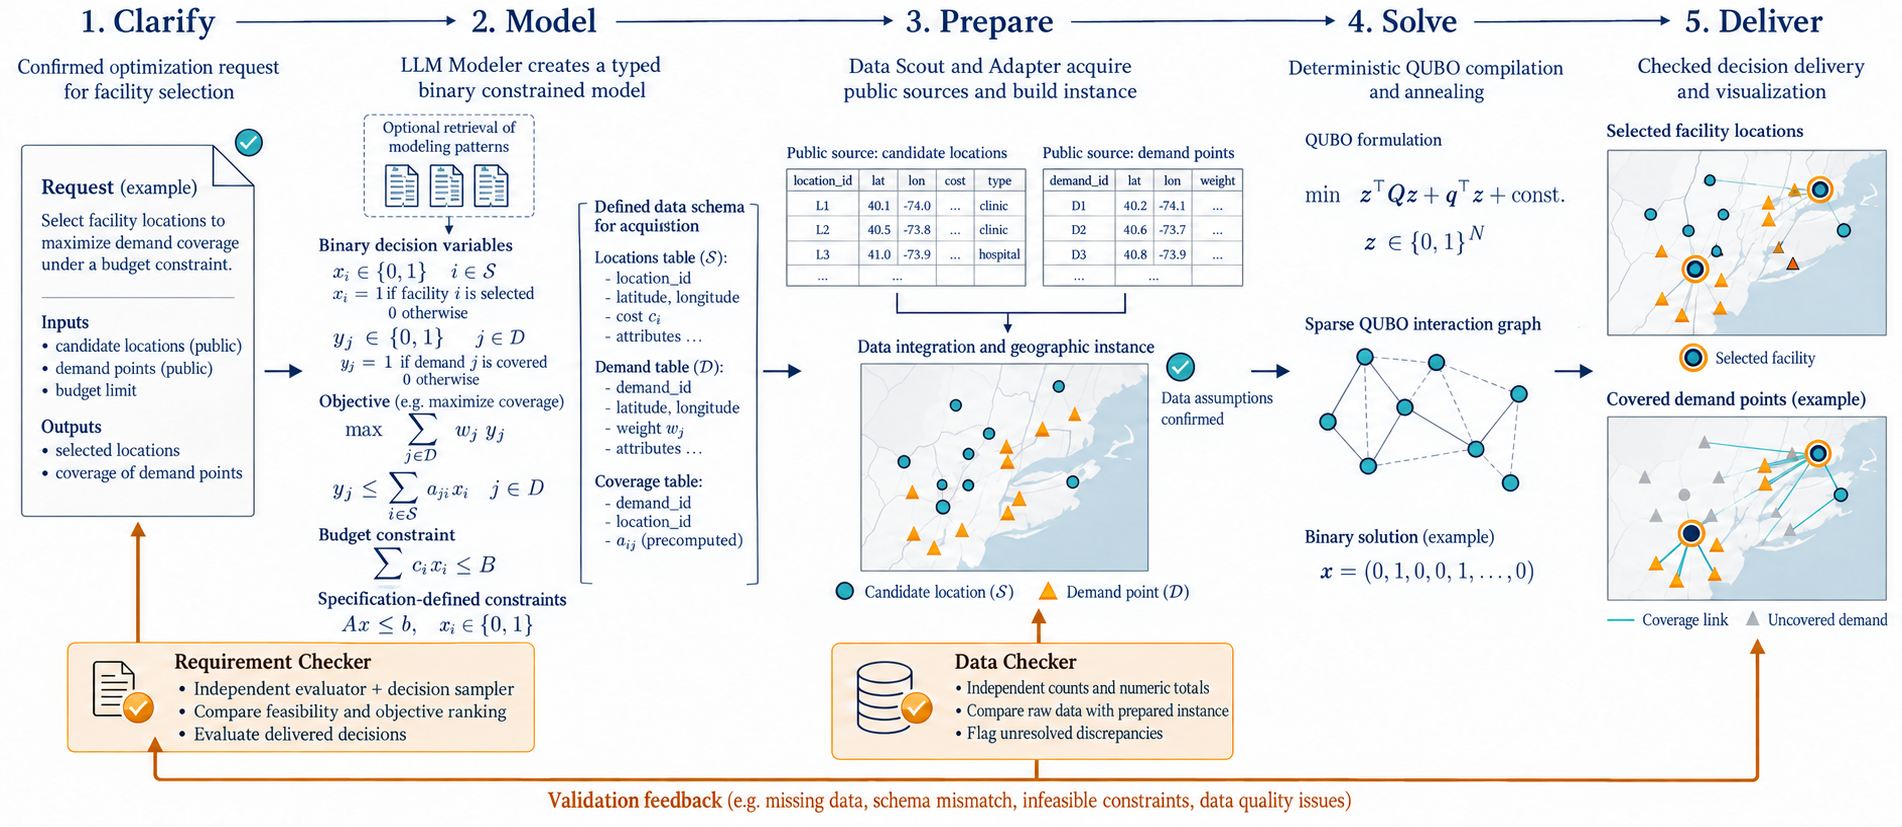
\includegraphics[width=\textwidth]{figures/workflow-illustrated.png}
\caption{Illustrative end-to-end facility-selection workflow. A confirmed request becomes a typed binary
model and schema, a prepared public-data instance, a QUBO and a checked decision. Coverage variables prevent
double-counting; QUBO variables include decision and encoding auxiliaries. Checker evidence supports bounded
repairs, not a guarantee of correctness. Tables, coordinates, maps and bit assignments are schematic examples.}
\label{fig:workflow}
\end{figure*}


\subsection{Local agent roles and executable control}
All runtime roles use Qwen3.6-35B-A3B (FP8), served by vLLM\cite{kwon2023vllm} on NVIDIA L40S GPUs. Agent
inference is local, while cloud solvers receive the submitted instance. Local serving does not make compute
free or guarantee that all data stays on the machine. The controller executes structured proposals, validates
outputs and enforces call limits. Per-call reasoning budgets and a retry without reasoning address empty answers.

The Clarifier drafts objectives, hard and soft constraints, data needs and assumptions, then asks bounded
questions. When clarification depends on external facts, code searches and fetches pages, and the agent revises
the draft with those passages. References are restricted to fetched pages or marked unverified.
The Modeler writes a data declaration, small-instance generator, binary-model builder and solution description.
Checks test JSON persistence, objective presence, structural constraint coverage, accidental penalty terms in
the original objective and small-instance feasibility. Failed attempts receive the previous code and specific
errors. A separate visualization task emits a bounded figure specification for deterministic rendering.
These structural checks cannot establish semantic correctness by themselves.

\subsection{Data acquisition and interpretation}
The data interface separates entity sets from parameters indexed by those sets. Declarations include source
class, type, unit, derivation and available period, geography and granularity. Code checks unique IDs, array
shapes, sparse-index membership, finite numeric values and declared ranges. Canonical spatial inputs use WGS84
latitude and longitude, and distances use metres. Fixed user settings are protected against data-level changes.

The Scout searches public-data catalogs and source pages. Implemented connectors include CKAN, Socrata,
Opendatasoft, ArcGIS Hub and the European data portal; supported WFS layers are requested as JSON in WGS84.
Catalog-provided or fetched links are used instead of guessed download URLs. Acquisition tries alternative
sources within bounded search and download attempts and retains errors.

The Adapter sees bounded table profiles and generates code operating on the full downloaded tables.
A preprocessing toolkit handles encodings, geospatial files, coordinate conversion, subtotal rows, stacked
periods and mixed administrative levels. Detected situations can require toolkit calls. For administrative
joins, parent districts can be propagated before filtering village rows; compound keys avoid matching by village
name alone. Row counts, duplicate keys, unmatched entities and source hashes are recorded by code.
Unknown metadata remains a review item. An explicitly reducible set can use weighted clustering; reduction is
not permitted when the confirmed request requires every original entity.

\subsection{Separate data and requirement checkers}
\label{sec:checkers}
Figure~\ref{fig:verificationlayers} shows two runtime checks and the separate evaluation judge.
When enabled, the Data Checker sees the request, schema and raw-table profiles, without Adapter code. It writes
an independent computation of expected counts and numeric totals. Prepared outputs are compared with these
aggregates, using a 0.5\% total tolerance with a unit-scale floor. Counts are skipped for declared reducible sets.
Disagreement is fed back to the Adapter; an unresolved mismatch is flagged for review. Checker-generation errors
are retained. Matching aggregates cannot detect every incorrect per-entity value or permutation.

The Requirement Checker sees the specification and data schema, without the formulation, and writes an
evaluator and decision sampler. Decision identities link model variables to entity IDs independently of bit
positions. Before solving, sampled valid and perturbed invalid decisions are checked against the model.
Decision variables are fixed, and a time-limited MILP optimizes remaining helper variables where supported;
the resulting feasibility and objective ranking are compared with the Checker. After solving, delivered
decisions are evaluated again. Timeouts and unsupported helper interactions are inconclusive.
Because both roles share a base LLM and schema, checker agreement is evidence, not a correctness guarantee.

\begin{figure*}[t]
\centering
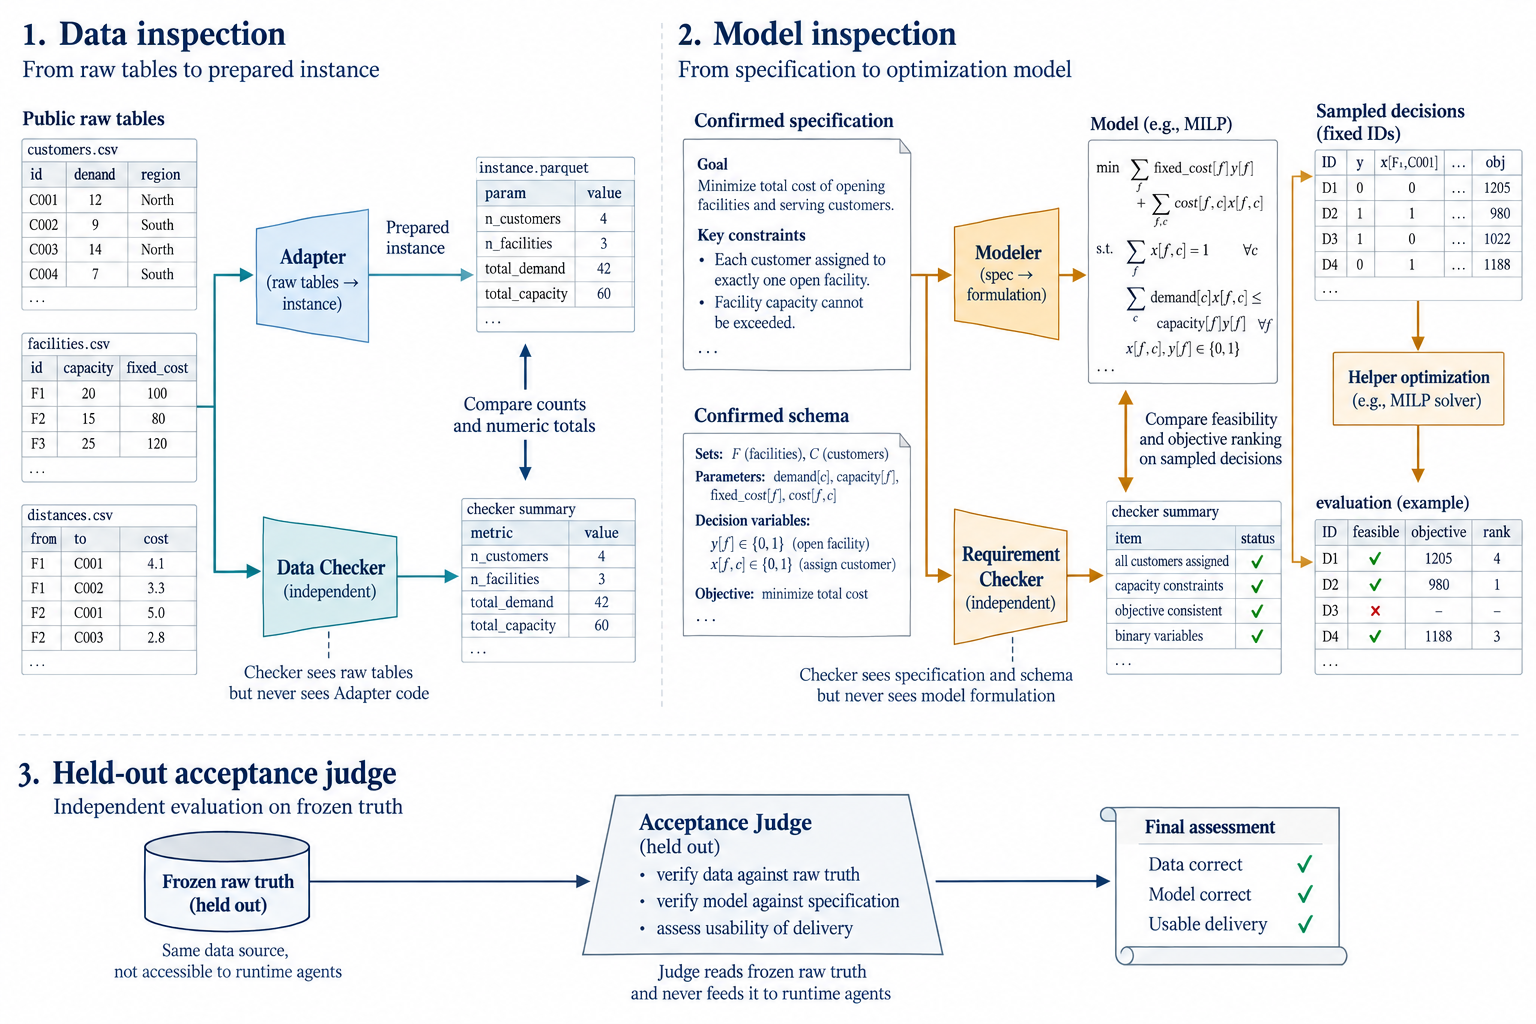
\includegraphics[width=\textwidth]{figures/verification-illustrated.png}
\caption{Illustrative data inspection, requirement inspection and external acceptance judging. Tables,
formulations, evaluation values and check marks are schematic examples, not experimental results.
Agents receive bounded raw-table profiles and write code that operates on full tables; the Requirement
Checker does not see the formulation. Helper optimization is used where supported. Checker agreement is
evidence rather than a correctness guarantee; held-out judge truth is not supplied to runtime agents.}
\label{fig:verificationlayers}
\end{figure*}


\subsection{Compilation, solving and recovery}
Equalities use squared penalties; inequalities use binary or unary slack, or approximate unbalanced
penalization\cite{montanez2024unbalanced}. Exclusion and implication constraints use pairwise penalties.
PyQUBO placeholders allow weights to change without recompiling the same encoding\cite{pyquboDocs}.
Explicit labels preserve decision and auxiliary indices. Encoded penalty diagnostics supplement original
constraint checks; incorrectly populated slack can give a penalty even for a feasible original decision.

The backend interface supports simulated annealing (SA), Compal GPU Annealer (CGA), Fujitsu Digital Annealer
(DA)\cite{aramon2019digital}, and D-Wave direct QPU or Leap Hybrid BQM. The experiments use SA, CGA and Leap
Hybrid. No direct-QPU experiment is reported; DA was blocked by an account usage limit.
The default policy is selected initially. Explicit alternatives include LLM tuning, rules, random search,
Optuna\cite{akiba2019optuna} and penalty-only searches. Bounds, parameter ranges and encoding-specific checks
reject invalid proposals. A single-flip penalty floor is a heuristic, not a proof of global-optimum preservation.
For large models, agents receive constraint families rather than every individual constraint.

Before annealing, a time-limited HiGHS preflight checks feasibility. Proven infeasibility avoids a solver call;
timeout remains unknown. A feasible conventional solution supplies a comparison baseline. For quadratic
objectives, bounded local improvement does not certify an optimum. If annealing has no feasible result or
trails a validated baseline beyond the configured tolerance, that baseline may be delivered with its source stated.

Evidence routes repairs to data preparation or modelling instead of treating every failure as a weak penalty.
An acquisition schema mismatch can trigger a new model and renewed preparation. Download failures do not
by themselves justify changing a model. Requirement-check disagreements can supply model-repair evidence.
Repairs are bounded, validated before activation and share the remaining solver budget. Comparisons on original
data protect existing formulas and fixed settings; changed requirements or unresolved substitutions need user
confirmation. These checks cannot prove that a repair preserves natural-language meaning.

Model code, data and provenance are versioned together. Generated code runs in separate processes with
timeouts, providing process isolation rather than a security sandbox. Supported penalty searches resume from
recorded histories, while changed-model or unresolved-call checkpoints are rejected. Saved solutions survive
visualization or explanation failures.

\subsection{Optional modelling-pattern retrieval}
The Modeler can select up to three general patterns by title from a local library and receive their text as
additional context. Repairs retain the selected IDs. This bounded retrieval supplies building blocks, not a
case-specific completed formulation. Its modelling-stage effect is distinct from retrieval of tuning knowledge;
no positive end-to-end retrieval effect is assumed.

\section{Problem-Level Ground-State Verification}
\label{sec:verification}
\subsection{Why reference bitstrings can misjudge a model}
QuantumQUBO Agent verifies small test cases by asking an LLM to translate human-stated solutions into reference
bitstrings in the generated formulation's variable layout\cite{mondal2026quantumqubo}. Enumeration accepts a
QUBO when its minimizers overlap with those references. The reference writer must count variables and populate
decision, slack and auxiliary bits without executing the model.

We audited all 33 failures in a local-model run with 67 successes on the 100-problem benchmark. Twelve failures
were shape mismatches. In at least seven, the generated test case had the wrong variable count; two arose from
model code and three remained undetermined. Six further failures concerned input-format mismatches and eleven
concerned argmin mismatches. A quadratic-assignment benchmark also stated an assignment costing 20 together
with an optimum of 12. Thus, failure against a generated reference need not indicate a wrong formulation.

\subsection{Verification in the language of the problem}
A case contains data $d$, the human-stated optimum $v^*$, an optional stated optimal solution and a shared
problem-level solution format. The generated builder includes a decoder. A separate Checker, written from the
problem statement without seeing the formulation, evaluates decoded decisions. Where a stated solution exists,
its evaluation must reproduce $v^*$ before the Checker is trusted on that case.

Let $G$ be the set of enumerated ground states. Acceptance requires
\begin{equation}
\begin{aligned}
 &\forall x\in G:\quad \mathrm{feasible}(\mathrm{decode}(d,x))\\
 &\qquad{}\land\ f(\mathrm{decode}(d,x))=v^*,
\end{aligned}
\end{equation}
with the implementation's numeric comparison tolerance. Checking every ground state rejects a degenerate QUBO
that also admits an invalid or non-optimal decision. Inconsistent reference/checker cases are marked
unverifiable rather than blamed on the model. Encodings beyond the enumeration threshold of 26 variables are
also unverifiable under this protocol. This exhaustive benchmark check is distinct from the sampled runtime
Requirement Checker in Section~\ref{sec:checkers}.

\subsection{Repeated benchmark results}
Table~\ref{tab:verification} retains unverifiable cases as a separate outcome. Five benchmarks failed under the
local bitstring protocol but succeeded in all three problem-level runs; three showed the reverse because their
ground states included non-optimal decisions. Of 16 unverifiable outcomes, ten exceeded the enumeration limit
and six reflected disagreement with benchmark references.

\begin{table}[t]
\centering\small
\caption{Results on 100 benchmarks. The original authors used remote models; local comparisons use the same locally served model.}
\label{tab:verification}
\begin{tabular}{@{}lrr@{}}\toprule
Protocol & Successes & Unverifiable \\
\midrule
Original authors' bitstring result & 68 & -- \\
Local bitstring run & 67 & -- \\
Problem-level, run 1 & 69 & 4 \\
Problem-level, run 2 & 72 & 6 \\
Problem-level, run 3 & 70 & 6 \\
\bottomrule\end{tabular}
\end{table}

The mean problem-level success rate is 70.3\% (range 69--72\%). Although temperature is zero, 27 benchmarks
changed outcome across repeated runs; 56 succeeded in all three and 17 in none. These observations support
repeated evaluation and recording per-problem outcomes. The protocols differ in both reference construction
and acceptance strictness, so their aggregate rates are not a clean causal estimate of one changed component.

\section{Experimental Evidence}
\label{sec:experiments}
We separate generated-model validation, solving frozen models and handling real data. Local benchmark and
synthetic-pipeline conditions use three repetitions; later backend comparisons also use three submissions per
condition. External repetitions are resubmissions without exposed hardware RNG seeds. Their search times are
not equivalent compute resources. No failed experiment is replaced by a simulated hardware result.

\subsection{Synthetic end-to-end modelling}
For twelve categories, we supplied one realistic request and ran clarification and modelling three times,
answering questions with the proposed defaults. The instances came from the generated synthetic-data function,
so this suite tests the pipeline rather than autonomous acquisition. All 36 clarifications converged and all
36 models passed validation; 35 produced a validated figure. Median pipeline time was 5.6 minutes.

One GPU solve per category reached the exact optimum in seven of nine categories with known references.
A portfolio instance had no feasible GPU result, and network design remained far from optimal.
Two development checks were initially wrong: a sorting detector rejected models with overlapping constraints,
and visualization was skipped when enumeration was impossible. Both were corrected and affected categories
rerun. These results concern the resulting evaluation configuration, not a frozen first-attempt success rate.

Mechanism observations explain some local-model failures. On a 1,680-variable scheduling model with 3,324
constraints, describing ten constraint families reduced tuning prompts from approximately 53k--54k to 2k--3k
tokens. Splitting model generation from visualization produced an EV-charger model and figure in two of three
runs. A reasoning cap with one retry without reasoning reduced empty Coder answers from 7/240 (2.9\%) to
5/521 (1.0\%). These observations are narrower than a controlled estimate of the value of every agent role.

\subsection{Routing scale and limits}
An LLM-generated single-vehicle routing model uses $n^2$ position variables. With ten-second CGA jobs, all
returned tours were feasible up to 60 stops (3,600 variables). Quality was exact up to ten stops and matched a
20-restart 2-opt reference up to 30 stops. Relative differences rose to 12.4\%, 27.2\% and 43.5\% at 40, 50 and
60 stops. The references are exact only at small sizes; larger references are feasible heuristics.
These are one-shot size measurements, not repeated evidence of an annealing advantage.

\subsection{Frozen-model backend comparisons}
The red-wine, 60-item knapsack and 80-item conflict-selection models were frozen before comparing defaults,
TPE penalty search and an LLM tuning agent. Each condition allowed at most three calls. SA used 60 reads and
300 sweeps; CGA used a three-second search limit. All 54 SA/CGA conditions produced feasible solutions.
The same three models and policies produced feasible results in all 27 Leap Hybrid conditions, using 72 actual
submissions. Every Hybrid call explicitly requested ten seconds; instances requiring a larger service minimum
were refused rather than assigned a longer time. Figure~\ref{fig:evidence} reports the observed mean gaps.

\begin{figure*}[t]
\centering
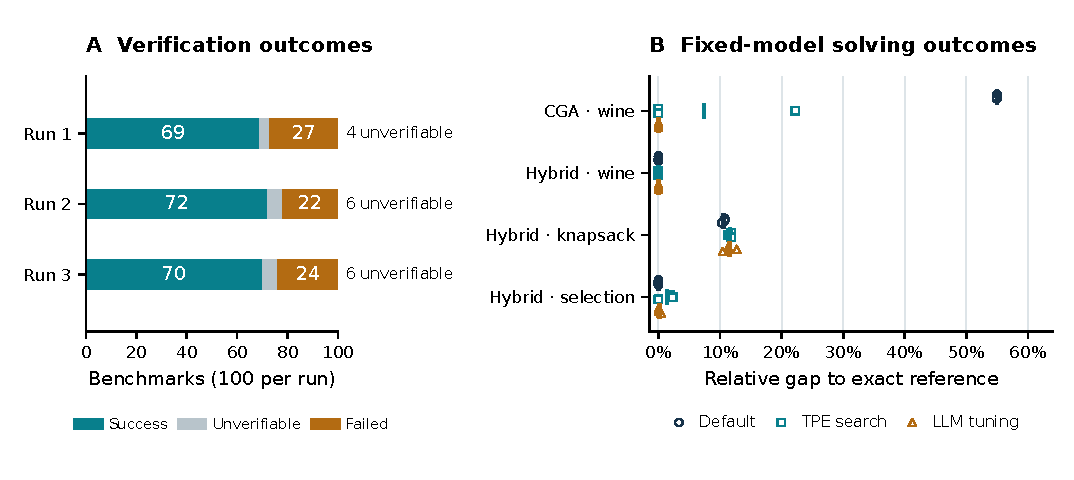
\includegraphics[width=\textwidth]{figures/evidence.pdf}
\caption{Recorded evaluation outcomes. Left: successes and unverifiable cases across three runs on the same
100 benchmarks; the remaining cases failed verification. Right: mean original-objective gaps on four selected
frozen-model/backend combinations, three repetitions per policy. Hollow markers show all three observed repetitions per condition; short vertical marks show their means. No confidence intervals are inferred.
CGA and Hybrid have different per-call limits; the plot does not establish a hardware advantage.}
\label{fig:evidence}
\end{figure*}


CGA defaults reached the reference on both non-wine models. On wine, mean gaps were 0.5495 for defaults,
0.0740 for TPE and 0.0000 for LLM tuning. Hybrid attained the wine reference under all three policies, but
knapsack mean gaps remained 0.1060, 0.1164 and 0.1149. These outcomes vary with model and backend.
Hybrid is not direct-QPU sampling, and its ten-second ceiling differs from CGA's three-second ceiling.
A real DA submission was rejected at the monthly account limit; no successful DA results are reported.

\subsection{Penalty search as a supporting component}
An earlier budget-matched SA comparison used 80 paired runs per policy. LLM variants reached mean gaps of
0.073--0.078 versus 0.084 for defaults, but defaults attained the optimum more often (38/80 versus 25--35/80).
Splitting tuning into diagnosis and refinement did not help ($p=0.10$), nor did retrieval of tuning knowledge
($p=0.17$). These results do not evaluate modelling-pattern retrieval.

In a separate eight-instance comparison with ten seeds and eight policies (640 SA runs), all runs returned
feasible results. Default weights had the lowest mean gap, 0.0932; penalty-only TPE, grid, cross-entropy and
sequential search had means 0.1080, 0.1070, 0.1372 and 0.1003. Paired Wilcoxon tests on eight instance-averaged
differences gave Holm-adjusted $p=0.03125$ for each of the four comparisons. Runs allowed six calls with 60
reads and 300 sweeps per call. This negative result supports keeping penalty search subordinate to data and
model validation, rather than claiming a generally superior tuning strategy.

\subsection{Real data: preparation and specified-source pilots}
The preprocessing toolkit reproduced Taipei's published village population from 63,315 rows containing ROC
years, stacked months, gender categories and mixed administrative levels, then joined official boundaries in
TWD97 coordinates. The cleaned total of 2,418,872 matched the published city total. Of 456 villages, 455 matched
by name; the final one required a variant-character match. An earlier transformation retained a city-total row
and doubled population, which aggregate provenance checks exposed. This is a toolkit validation, not autonomous
end-to-end acceptance.

A specified-source wine pilot used all 1,599 UCI records\cite{uciWine}. The local LLM wrote the model and
Adapter; selecting five features achieved objective 0.7497088247 after four SA calls, matching enumeration of
all 2,048 assignments. The successful fresh run used approximately 64 seconds and 20,596 LLM tokens.
A recovered UCI wholesale-customer pilot\cite{uciWholesale} formed three equal groups from 24 sampled records,
with objective 856.8319 versus 1021.7818 for a feasible baseline (16.1\% lower).
A recovered karate-club case delivered two groups of 17 with 17 cut edges from the baseline because annealing
returned 22. These pilots used manually specified inputs or independent case-specific checks; some reused
models or caches. They do not establish unrestricted autonomous data acquisition or a prospective success rate.

\subsection{Autonomous acceptance protocol and remaining execution}
A new runner starts without saved models, instances or LLM cache. Agents receive a request and fixed user
answers specifying settings, without formulas or field names. Each configuration must find and download data.
Three tasks are defined: five Taipei charger sites maximizing population covered within one kilometre;
a tour of all YouBike stations within 500 metres of a specified point; and three equal-size groups of eligible
AED inspection locations. The charger task preserves all villages and prohibits sampling.

An external case-specific judge uses frozen raw-data truth withheld from the runtime agents. It checks
one-to-one entity coverage, coordinates and measured values; tests model feasibility and objective ranking on
30 sampled decisions; and verifies delivered requirements and quality within 10\% of a feasible reference where
available. The ranking threshold is 0.9. Data correctness, model correctness and usable delivery are separate
outcomes; joint success requires all three. Judge failures and unsupported representations are retained.

Five configurations compare a direct LLM, a structured workflow, added independent checkers, added cross-stage
repair and added modelling-pattern retrieval. Three repetitions on three tasks require 45 runs. An optional
comparison disables only clarification web lookup, giving 54 runs. Common ceilings include four model attempts,
three solver calls using CGA defaults and bounded repairs. The direct configuration has different acquisition
tools and download limits, so it compares complete systems rather than isolating agent count. Automated
confirmations are fixtures rather than observed user-effort measurements.

Existing development records span changing code and prompts and include both successful YouBike deliveries
and upstream failures. They are not pooled into a success rate. Code, prompts, cases and truth are hashed for
new frozen batches; the repeated comparison remains incomplete. Consequently, no end-to-end advantage for
multi-agent coordination, checking, repair or modelling retrieval is reported here.

\section{Discussion and Limitations}
The current evidence supports distinct claims. Repeated small benchmarks evaluate formulation checking;
the synthetic suite tests workflow connections; frozen models test solver behaviour; specified-source pilots
test particular data and modelling paths. None substitutes for repeated autonomous real-data acceptance.
The offline suite passes 146 tests, including schema, checker, recovery and checkpoint fixtures, but test counts
do not measure semantic correctness or live acquisition reliability.

Runtime checkers can share LLM and schema errors. Matching counts and totals can hide per-entity mistakes,
and sampled requirement checks cannot verify every state. Exhaustive ground-state checking is limited to 26
variables. A generated objective can still replace the requested objective with a weaker surrogate.
Model repair and data substitution may require user judgment, even when structural checks pass.

Hardware comparisons contain three repetitions per condition and allocate different service budgets.
They establish working submissions and instance-specific outcomes, not quantum advantage, lower total cost or
a generally preferable backend. Conventional baselines can be the delivered result, as in the network pilot.

\section{Conclusion}
We presented a local-LLM workflow connecting requirements, typed data preparation, modelling, annealing and
checked delivery. Separate validation of data, model meaning and solver feasibility supports bounded repair.
Ground-state verification exposes reference-bitstring failures. The next step is a frozen autonomous real-data
comparison measuring the incremental effects of checking, repair and retrieval.

\IEEEtriggeratref{7}
\bibliographystyle{IEEEtran}
\bibliography{references}
\end{document}
